% Asking Is (Almost) All You Need -- Team The Misfits, Round 2 technical report.
% Build: tectonic paper.tex   (or pdflatex paper.tex twice; or upload this folder to Overleaf)
\documentclass[10pt]{article}

\usepackage[T1]{fontenc}
\usepackage[utf8]{inputenc}
\usepackage{mathptmx}            % Times, as in the NeurIPS style
\usepackage[letterpaper,textwidth=5.5in,textheight=9in,top=1in]{geometry}
\usepackage{amsmath,amssymb}
\usepackage{booktabs,tabularx,multirow}
\usepackage{graphicx}
\usepackage[font=small,labelfont=bf,skip=4pt]{caption}
\usepackage{microtype}
\usepackage{xcolor}
\usepackage{enumitem}
\usepackage{tikz}
\usetikzlibrary{positioning,arrows.meta,fit,backgrounds}
\usepackage[colorlinks=true,linkcolor=black,citecolor=black,urlcolor=blue!50!black]{hyperref}

\setlist{nosep,leftmargin=1.4em}
\setlength{\parskip}{3pt}
\setlength{\parindent}{0pt}
\emergencystretch=2.5em
\newcommand{\msmi}{\textsc{msmi}}
\newcommand{\full}{\texttt{full}}
\newcommand{\ship}{\texttt{full\_person\_learn}}
\newcommand{\ci}[2]{[$#1$,\,$#2$]}
\definecolor{cblue}{HTML}{2A78D6}
\definecolor{corange}{HTML}{EB6834}

\title{\Large\bfseries Asking Is (Almost) All You Need:\\Sequential Reciprocal Matching under Uncertainty}
\author{}
\date{}

\begin{document}
\maketitle
\vspace{-3.2em}
\begin{center}
\begin{tabular}{@{}c@{\hspace{2.2em}}c@{\hspace{2.2em}}c@{}}
\textbf{Rishi Mehrotra}$^{*}$ & \textbf{Siddharth Malkania}$^{*}$ & \textbf{Krishna Vallabha Goswami}$^{*}$ \\
Team The Misfits & Team The Misfits & Team The Misfits
\end{tabular}\\[0.3em]
{\footnotesize $^{*}$Equal contribution. Author order follows the Round~1 proposal.}\\[0.5em]
{\small\itshape The Sequential Matching Problem: Applied Machine Learning Programme \& Hackathon,\\ Romeo \& Juliet Ltd.\ $\times$ IIT Madras. Round 2 technical report, October 2026.}\\[0.3em]
{\small Code, results and reproduction commands: \url{https://github.com/krishnavallabha/BRVM}}
\end{center}

\begin{abstract}
\noindent
Each simulated day, a matchmaking policy must decide which clarifying questions to ask under a fixed budget and which feasible, non-overlapping introductions to make, in a changing pool with incomplete profiles and delayed, selective feedback. The objective is \emph{mutual second-meeting intention} (\msmi) per 100 arrived members, and a single invalid action in any of 120 private episodes disqualifies an entry. Our Round~1 proposal, Bayesian Reservation-Value Matching, assumed that lookahead, exploration and rich outcome models would carry the score. In Round~2 we \emph{measured before modelling}.
\begin{itemize}[leftmargin=1.2em]
\item We built an exact expected-\msmi{} yardstick from the public simulator's mechanics, validated it against realised outcomes on 360 episodes, and cut paired evaluation noise about $10\times$.
\item The yardstick shows that selection headroom is small: a matcher that knows every true probability gains only about $+7\%$ over greedy. Clarification is the dominant lever: without questions the score falls by $71\%$.
\end{itemize}
Our shipped policy combines partner-count question ordering, cheap goal and pace questions, and maximum-cardinality matching whose tie-breaks use observed soft-field fit, a hierarchical empirical-Bayes model of each person's responsiveness and acceptance, and an online Bayesian fit model. On fresh, reserved seeds it improves expected \msmi{} over the supplied greedy baseline by $+0.0115$ \ci{+0.0044}{+0.0186} per 100 members ($+3.0\%$), with no scenario family clearly worse. It is valid in every episode we ran, including the official container protocol (median $0.95$\,s per call).

We also report negative results. Waiting for better matches, whether by simple reservation or by our own sampled-future prices, never helps. The models are calibrated but weakly informative. And in sparse graphs the choice among equally large matchings measurably affects future availability.
\end{abstract}

% ======================================================================
\section{Introduction}

Reciprocal recommendation differs from ordinary recommendation in three ways:
\begin{itemize}
\item both sides must accept;
\item every introduction occupies both people for days;
\item outcomes arrive late and only for the pairs one chose to introduce.
\end{itemize}
The Sequential Matching Problem turns this into a 60-day sequential decision task. Each day has two phases: an \emph{ask} phase, which spends a 12-unit clarification budget on hard-constraint bundles (3 units) or single soft fields (1 unit), and a \emph{match} phase, which proposes a set of disjoint, reciprocally feasible pairs. Scoring is purely technical: the equal-weight mean over six scenario families of \msmi{} per 100 arrived members, with ties broken by coverage, mutual acceptances, lower clarification cost and lower inference time.

Our Round~1 proposal, Bayesian Reservation-Value Matching (BRVM), committed to a sophisticated design:
\begin{itemize}
\item a staged hierarchical outcome model;
\item reservation values estimated as LP duals over sampled futures;
\item Thompson sampling;
\item value-of-information clarification;
\item a scenario-aware meta-policy.
\end{itemize}
This report documents what happened when that design met measurement. Our contributions are:
\begin{enumerate}
\item \textbf{A validated low-noise yardstick.} Exact expected \msmi{} per introduction, computed from simulator truth \emph{for evaluation only}. It agrees with realised outcomes (ratio $0.91$, $z=-1.53$, 360 episodes) and cuts the paired standard deviation from $0.44$ to $0.04$ per episode (Section~\ref{sec:yardstick}).
\item \textbf{A headroom analysis} that bounds what any allocation rule can gain and locates the remaining value (Section~\ref{sec:headroom}).
\item \textbf{A simple, robust, confirmed policy.} Each component is ablated, and the policy is confirmed twice on reserved seeds: $+0.0092$ and then $+0.0115$ over greedy (Sections~\ref{sec:method}--\ref{sec:results}).
\item \textbf{An observable-only Bayesian layer.} A hierarchical empirical-Bayes person model and an online fit model, with a calibration study. They add $+0.0041$ \ci{+0.0012}{+0.0071} on fresh seeds and adapt to shifted outcome weights without recognising the scenario (Section~\ref{sec:bayes}).
\item \textbf{Honest answers to the reviewers' questions}, including negative results for our own Round~1 ideas (Section~\ref{sec:questions}).
\end{enumerate}

% ======================================================================
\section{Problem setting}\label{sec:setting}

A pool of $n=200$ synthetic members arrives over days $0$--$20$; about $70\%$ arrive on day $0$ and about $12\%$ exit at a random day between $22$ and $60$.

\textbf{Fields.} Each member has public attributes (age, gender, zone), hard fields $\mathcal{H}$ (age range, genders sought, relationship structure, smoking, children, zones, schedule) and soft fields $\mathcal{S}$ (goal, pace, lifestyle, conversation style, and others). Each field is \emph{observed}, \emph{not asked} or \emph{declined}.

\textbf{Feasibility.} A pair $(i,j)$ is \emph{feasible} iff every hard field of both members is known and every reciprocal check passes. Unknown never means compatible, and a declined hard field makes a member permanently ineligible. On day $t$ the policy may introduce any matching $M_t$ on the graph of feasible, available, never-introduced pairs. After an introduction both members are busy for 8 days, and longer after a mutual acceptance.

\textbf{Outcomes.} For each introduction the simulator draws, in order:
\begin{itemize}
\item a response from each member (rate $r_i \in [0.55, 0.98]$);
\item acceptance, which depends on a person-level bias, soft-field fit and a shared pair shock;
\item a date within 30 days ($p=0.78$, later in the \emph{delayed} family);
\item two second-meeting answers within 3 days.
\end{itemize}
An introduction counts as an \msmi{} when all of these succeed. For an episode with $N$ members arrived by day 59, the score is $100\,\#\msmi/N$, and the primary metric averages over 20 private seeds within each of six families (\emph{standard, sparse geography, cold start, delayed dates, shifted outcome weights, changing response conditions}), then over families.

\textbf{Observations.} The policy sees only the request JSON: current fields and statuses, availability, past introductions and observed feedback. It never sees $r_i$, biases or seeds.

% ======================================================================
\section{Measuring before modelling}\label{sec:yardstick}

\paragraph{Expected-\msmi{} yardstick.}
Realised \msmi{} is extremely noisy: about $0.7\%$ of introductions succeed, and an episode has about 1--2 successes. Because the simulator is public, we can compute each introduction's exact success probability for \emph{evaluation} (never in the policy):
\begin{equation}
p_{ij} \;=\; r_i^2 r_j^2 \cdot 0.78\,\pi_{30} \cdot 0.36 \;\mathbb{E}_{\epsilon}\!\big[\sigma(\ell_{ij}+\epsilon)\,\sigma(\ell_{ji}+\epsilon)\,\sigma(s_i+\epsilon+g_{ij})\,\sigma(s_j+\epsilon+g_{ij})\big],
\end{equation}
where:
\begin{itemize}
\item $\ell_{ij}$ is $i$'s acceptance logit for $j$;
\item $s_i$ is $i$'s second-meeting logit, with $g_{ij}$ its goal-match boost;
\item $\epsilon\sim\mathcal{N}(0,0.45^2)$ is the shared pair shock, integrated by 40-point Gauss--Hermite quadrature;
\item $\pi_{30}$ is the probability that the date falls inside 30 days;
\item $0.36=(3/5)^2$ is the probability that both second-meeting answers are on time.
\end{itemize}
The response rate appears squared per person, because each member must answer both the introduction and the second-meeting question. Summing $p_{ij}$ over a policy's introductions gives its expected \msmi.

\paragraph{Validation.} On 360 greedy episodes (seeds 201--260, all families) expected and realised totals agree: $265.7$ vs $241$ events (ratio $0.91$, $z=-1.53$), and every family's 95\% CI on the per-episode difference contains $0$.

\paragraph{Variance reduction.} The paired difference between two policies on identical worlds has a per-episode SD of $0.44$ when measured by realised \msmi{}, but $0.041$ when measured by expected \msmi{}. That is a $10\times$ reduction, or about $100\times$ fewer seeds for the same power. Every comparison in this report is paired and uses expected \msmi{}; realised values are reported alongside.

\subsection{How much is there to gain?}\label{sec:headroom}
On seeds 201--205 the expected \msmi{} per 100 members is $0.348$ for greedy and $0.362$ for random feasible selection. A greedy matcher that knows every true $p_{ij}$ reaches $0.360$, and a maximum-weight matching on the true $p_{ij}$ reaches $0.372$. \textbf{A perfect-information myopic allocator gains only about $+7\%$.} Removing all questions loses about $70\%$.

The reason is structural. The feasible graph is tiny (about $2.5$ partners per member), and about $34\%$ of members decline a hard field, which caps coverage at about $0.36$.

Figure~\ref{fig:headroom} decomposes the value of all feasible pairs under our policy. Of the value left on the table, about $0.07$ per 100 members comes from pairs whose members were both present but never scheduled. Drift timing losses are negligible ($0.004$). Across feasible pairs, the variance of $\log p_{ij}$ is explained $24\%$ by response rates, $27\%$ by acceptance and second-meeting tendencies, and $36\%$ by goal match ($11\%$ in the shifted-weights family). \emph{The signal is mostly about people, not pairs.}

\begin{figure}[t]
\centering
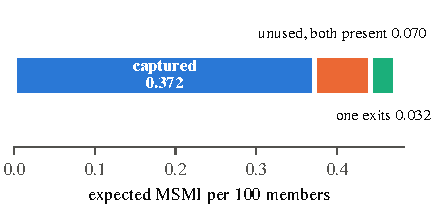
\includegraphics[width=0.62\linewidth]{figures/fig_headroom.pdf}
\caption{Where the value of feasible pairs goes under \full{} (seeds 201--215, all families). Most feasible value is captured. The largest recoverable pool is pairs whose members were both present but never scheduled.}
\label{fig:headroom}
\end{figure}

% ======================================================================
\section{Method}\label{sec:method}

Figure~\ref{fig:arch} shows the daily loop. Normalisation, modelling and allocation are kept separate, as the specification recommends. Every component is a configuration switch, so the supplied baselines, our policy and every ablation run through the same code.

\begin{figure}[t]
\centering
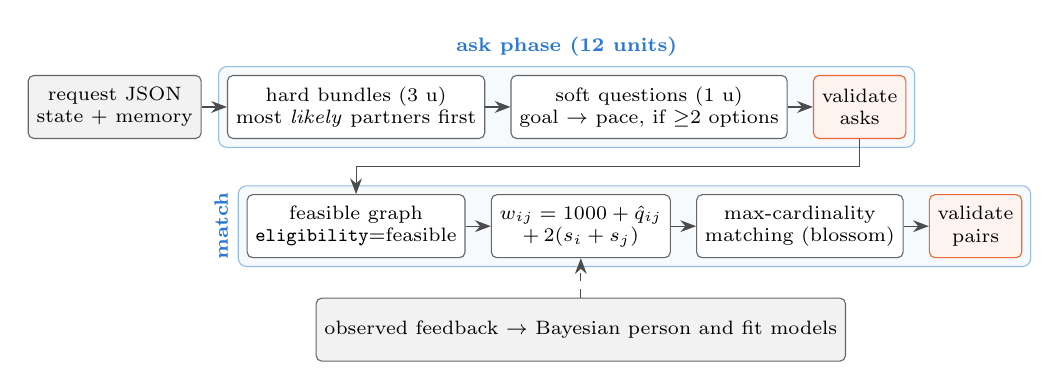
\begin{tikzpicture}[font=\scriptsize, node distance=3.5mm and 3.2mm,
  box/.style={draw=black!60, rounded corners=2pt, align=center, inner sep=3pt, minimum height=8mm, fill=white},
  io/.style={box, fill=black!5}, chk/.style={box, draw=corange, fill=corange!8},
  arr/.style={-{Stealth[length=2mm]}, black!70}]
\node[io] (req) {request JSON\\state + memory};
\node[box, right=of req] (hard) {hard bundles (3 u)\\most \emph{likely} partners first};
\node[box, right=of hard] (soft) {soft questions (1 u)\\goal $\rightarrow$ pace, if $\geq$2 options};
\node[chk, right=of soft] (v1) {validate\\asks};
\node[box, below=7mm of hard] (graph) {feasible graph\\\texttt{eligibility}$=$feasible};
\node[box, right=of graph] (w) {$w_{ij}=1000+\hat q_{ij}$\\$+\,2(s_i+s_j)$};
\node[box, right=of w] (bl) {max-cardinality\\matching (blossom)};
\node[chk, right=of bl] (v2) {validate\\pairs};
\node[io, below=5mm of w] (fb) {observed feedback $\rightarrow$ Bayesian person and fit models};
\draw[arr] (req) -- (hard); \draw[arr] (hard) -- (soft); \draw[arr] (soft) -- (v1);
\draw[arr] (v1.south) |- ++(0,-3.5mm) -| (graph.north);
\draw[arr] (graph) -- (w); \draw[arr] (w) -- (bl); \draw[arr] (bl) -- (v2);
\draw[arr, dashed] (fb) -- (w);
\begin{scope}[on background layer]
\node[fit=(hard)(soft)(v1), draw=cblue!50, fill=cblue!4, rounded corners=3pt, inner sep=3pt, label={[font=\scriptsize\bfseries,cblue]above:ask phase (12 units)}] {};
\node[fit=(graph)(w)(bl)(v2), draw=cblue!50, fill=cblue!4, rounded corners=3pt, inner sep=3pt, label={[font=\scriptsize\bfseries,cblue]left:\rotatebox{90}{match}}] {};
\end{scope}
\end{tikzpicture}
\caption{One simulated day. Asks are chosen, validated and resolved. The match phase then builds the feasible graph and solves a maximum-cardinality weighted matching. The weight keeps cardinality first, so models only break ties. Every output passes an independent validator.}
\label{fig:arch}
\end{figure}

\paragraph{Safety shell.} Validity is all-or-nothing, so the shell was built and tested before any model. It:
\begin{itemize}
\item re-checks every ask (available member, legal field, never observed or declined, no duplicates, budget) and every pair (\texttt{kit.eligibility}, availability, no repeats, nobody twice), and drops failures;
\item runs the policy under a 3\,s soft limit;
\item makes the match fallback deadline-aware: past 4.5\,s it returns no pairs instead of recomputing greedy;
\item checks memory for size and finiteness.
\end{itemize}
A 36-test suite fuzzes empty pools, all-unknown and all-declined fields, exhausted graphs, malformed memory, and choosers that raise, return garbage or hang. Disabling the validators makes 30 sub-tests fail.

\paragraph{Clarification.} Hard bundles go to candidates (available, a hard field not asked, none declined) ranked by \emph{likely partner count}: the number of other available members not yet introduced whose pair status is anything but \emph{infeasible}. Unknown fields therefore do not block. Arrivals in the last 3 days get a $+10$ bonus, tuned over $\{0,10,25,50\}$ on development seeds. Left-over budget asks \texttt{relationship\_goal} and then \texttt{relationship\_pace}, only for members with at least two feasible partners, since a soft answer can only change a choice when there is more than one option.

\paragraph{Allocation.} Each day we solve
\begin{equation}
M_t=\arg\max_{M\in\mathcal{M}(G_t)} \sum_{(i,j)\in M} \big(1000 + \hat q_{ij} + 2\,(s_i+s_j)\big),
\end{equation}
where $\mathcal{M}(G_t)$ is the set of matchings of the feasible graph $G_t$, solved with Edmonds' blossom algorithm~\cite{edmonds1965paths} (maximum-cardinality, maximum-weight). The base weight of $1000$ guarantees that cardinality is never traded for quality.

The blossom routine is vendored verbatim from NetworkX~\cite{hagberg2008networkx}, BSD-3. Importing the full library cost about $0.93$\,s on every call, because the policy process restarts per call. The vendored copy is identical on 6{,}000 random graphs and on full policy episodes.

% ======================================================================
\subsection{Observable-only Bayesian layer}\label{sec:bayes}

\paragraph{Person model.} For member $i$, let $(a_i, n_i)$ count answered vs total \emph{resolved} response opportunities, from introductions and second-meeting questions, and $(y_i, m_i)$ count yes answers among introduction responses.

Only opportunities whose answer window has closed are counted. A response appears 1--7 days after an introduction, but a non-response only at the 7-day deadline, so counting open opportunities inflated every response rate (calibration showed $0.9$ predicted vs $0.7$ observed).

We place Beta priors centred on the pool rate $\bar r$ with strength $\kappa$, and \emph{average} over $\kappa$ instead of picking one (hierarchical empirical Bayes~\cite{robbins1956empirical,gelman2013bayesian}):
\begin{equation}
\mathbb{E}[f(r_i)\mid\text{data}] \;=\; \sum_{\kappa\in K} w_\kappa\, \mathbb{E}_{\mathrm{Beta}(\bar r\kappa + a_i,\,(1-\bar r)\kappa + n_i - a_i)}[f],
\qquad
w_\kappa \propto \prod_{k}\frac{B(\bar r\kappa+a_k,(1-\bar r)\kappa+n_k-a_k)}{B(\bar r\kappa,(1-\bar r)\kappa)},
\end{equation}
over a log-spaced grid $K=\{2,\dots,400\}$, with $w_\kappa$ the beta-binomial marginal likelihood. With about two observations per member that likelihood is flat, and a single best $\kappa$ jumped between 8 and 400 from episode to episode; averaging stabilises the shrinkage. The person score is
\[
s_i=\log\mathbb{E}[r_i^2]+\log\mathbb{E}[\text{acc}_i]
\]
relative to a member with no data. The square mirrors the outcome structure of Section~\ref{sec:yardstick}.

\paragraph{Fit model.} A Bayesian logistic regression of a yes answer on soft-field agreement features ($+1$ equal, $-\tfrac12$ different, $0$ unknown), fitted by MAP with Newton steps. Its prior means are our hand-set weights divided by 4: goal $+3/{-1.5}$, pace $+1.5/{-0.75}$, and small lifestyle and conversation terms. With no data, $\hat q$ equals the hand-set fit exactly; with data, it adapts.

\paragraph{Sampled-future slot prices (tested, not shipped).} Member $i$'s price is
\[
\log\!\Big(1+\frac{\text{remaining feasible partners}+\text{expected future partners}}{\text{remaining slots}}\Big),
\]
where future partners are the recent arrival rate times days left times the share of resolved profiles feasible with $i$ (the sample average over resampled observed profiles), and remaining slots are days left divided by 8. It enters the weight as $\lambda(\text{price}_i+\text{price}_j)$.

% ======================================================================
\section{Experimental protocol}\label{sec:protocol}

\begin{itemize}
\item \textbf{Seeds.} Development and all tuning on seeds 201--260. Seeds 301--340 were reserved for confirming \full{}, and 341--380 for confirming the Bayesian layer; each set was used once, after the design was frozen. Public seeds 101--103 were used only to reproduce the published baselines.
\item \textbf{Baselines.} The supplied greedy, no-clarification and random-feasible policies, on identical seeds and all six families.
\item \textbf{Keep rule, fixed in advance.} A component is kept only if its paired difference against the current best is positive overall, no family's 95\% CI lies entirely below zero, and no episode is invalid.
\end{itemize}

% ======================================================================
\section{Results}\label{sec:results}

\begin{table}[t]
\centering\small
\caption{Official evaluator, real subprocess protocol, public seeds 101--103 $\times$ 6 families (18 episodes per policy, all valid). Per-episode means. Realised \msmi{} at this scale rests on 10--14 events per policy; the expected column is far less noisy.}
\label{tab:official}
\setlength{\tabcolsep}{4pt}
\begin{tabular}{lccccccc}
\toprule
Policy & Realised & Expected & Intros & Mutual acc. & Coverage & Wait med./p90 & Ask cost \\
\midrule
greedy & 0.389 & 0.373 & 79.8 & 11.00 & 0.372 & 4 / 16 & 207 \\
random & 0.278 & 0.370 & 80.5 & 10.67 & 0.377 & 5 / 16 & 207 \\
no\_asks & 0.139 & 0.116 & 24.3 & 3.50 & 0.143 & 0 / 13 & 0 \\
\full{} (core) & 0.278 & 0.362 & 78.5 & 11.94 & 0.375 & 4 / 16 & 220 \\
\textbf{\ship{}} & 0.306 & 0.373 & 79.9 & 11.67 & \textbf{0.376} & 4 / 16 & 219 \\
\bottomrule
\end{tabular}
\end{table}

\paragraph{Baselines and the official run.} Table~\ref{tab:official} reports the official protocol. Two observations stand out:
\begin{itemize}
\item Our policies produce \emph{more} mutual acceptances and dates than greedy, but at this scale they lost some of the final second-meeting draws.
\item In expectation, the shipped policy ties greedy on these three seeds. Three seeds cannot resolve effects of about $1\%$; the reserved-seed confirmations can.
\end{itemize}

\paragraph{Confirmation on reserved seeds.} Table~\ref{tab:confirm} and Figure~\ref{fig:families} give the evidence.
\begin{itemize}
\item On 301--340 the core policy \full{} beats greedy by $+0.0092$ \ci{+0.0011}{+0.0174}.
\item On fresh seeds 341--380 the shipped policy beats greedy by $+0.0115$ \ci{+0.0044}{+0.0186}, a $+3.0\%$ improvement. It is clearly better in the cold-start, delayed and changing-response families, positive in two others, and tied in sparse geography, where about 22 introductions per episode leave nothing to choose between.
\end{itemize}

\begin{table}[t]
\centering\small
\caption{Paired expected \msmi{} per 100 members on reserved seeds (240 episodes per policy, all valid), with 95\% CIs on the per-seed paired difference.}
\label{tab:confirm}
\setlength{\tabcolsep}{3.5pt}\footnotesize
\begin{tabular}{llccc}
\toprule
Seeds & Policy & Expected & vs greedy & vs \full{} \\
\midrule
\multirow{4}{*}{301--340} & greedy & 0.3841 & --- & \\
 & random & 0.3864 & $+0.0024$ \ci{-0.003}{+0.008} & \\
 & no\_asks & 0.1109 & $-0.2732$ \ci{-0.290}{-0.257} & \\
 & \full{} & 0.3933 & $\mathbf{+0.0092}$ \ci{+0.0011}{+0.0174} & --- \\
\midrule
\multirow{5}{*}{341--380} & greedy & 0.3779 & --- & $-0.0073$ \\
 & \full{} & 0.3852 & $+0.0073$ \ci{+0.0009}{+0.0138} & --- \\
 & \;+ person model & 0.3888 & $+0.0109$ & $+0.0036$ \ci{+0.0011}{+0.0061} \\
 & \;+ fit model & 0.3872 & $+0.0093$ & $+0.0020$ \ci{-0.0003}{+0.0042} \\
 & \;\textbf{+ both (shipped)} & \textbf{0.3894} & $\mathbf{+0.0115}$ \ci{+0.0044}{+0.0186} & $\mathbf{+0.0041}$ \ci{+0.0012}{+0.0071} \\
\bottomrule
\end{tabular}
\end{table}

\begin{figure}[t]
\centering
\begin{minipage}[t]{0.49\linewidth}\centering
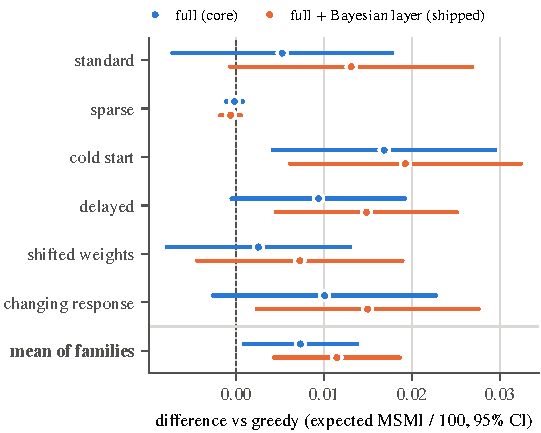
\includegraphics[width=\linewidth]{figures/fig_families.pdf}
\caption{Per-family gains over greedy on fresh seeds 341--380. The Bayesian layer lifts every family except the sparse one, where every policy ties.}
\label{fig:families}
\end{minipage}\hfill
\begin{minipage}[t]{0.49\linewidth}\centering
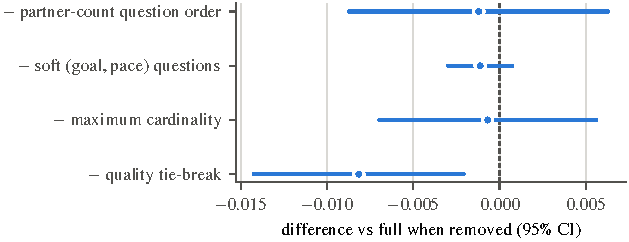
\includegraphics[width=\linewidth]{figures/fig_ablation.pdf}
\caption{Remove-one ablations of \full{} (seeds 301--340). Only removing the soft-fit-aware tie-break is clearly harmful; the other components substitute for each other.}
\label{fig:ablation}
\end{minipage}
\end{figure}

\paragraph{Ablations.} Figure~\ref{fig:ablation} shows the remove-one ablations.
\begin{itemize}
\item The load-bearing design claim is that \emph{allocation must use observed soft-field agreement}. Unit-weight maximum matching loses the whole gain ($-0.0082$ \ci{-0.0142}{-0.0021}).
\item Question order, soft questions and maximum cardinality are largely substitutes: any two of them recover about $+0.008$ over greedy. That is consistent with the low ceiling of Section~\ref{sec:headroom}.
\item Broad soft questioning (every field) matches the narrow design inside \full{} ($-0.0004$) at $2.7\times$ the ask cost, which is a tie-breaker, so the narrow design ships.
\end{itemize}

\paragraph{The Bayesian layer and calibration.} Figure~\ref{fig:cal} shows reliability diagrams for about 13{,}000 decision-time predictions.
\begin{itemize}
\item All three models are monotone and beat a pool-rate baseline: Brier skill $+0.7\%$ for response, $+0.55\%$ for acceptance and $+0.15\%$ for fit.
\item The fit model gains $+1.7\%$ skill in the shifted-weights family, where pace outweighs goal. It adapts without being told the family.
\item The tails remain overconfident, which is expected with two to three observations per person. The two fixes in Section~\ref{sec:bayes} were found through this diagnostic.
\end{itemize}

\begin{figure}[t]
\centering
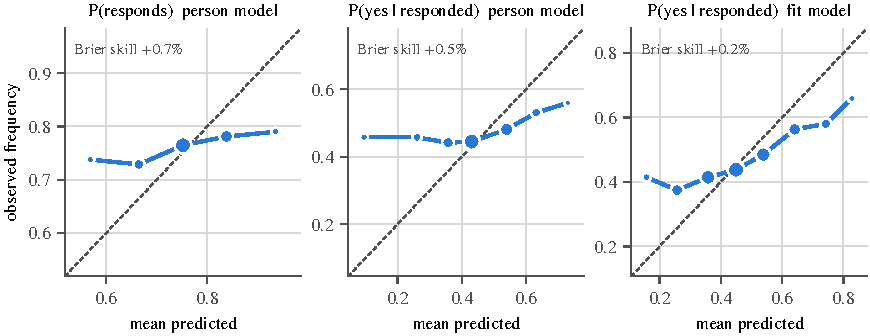
\includegraphics[width=\linewidth]{figures/fig_calibration.pdf}
\caption{Calibration of the observable-only models at decision time (seeds 201--215, about 13{,}000 predictions; marker area $\propto$ bin size).}
\label{fig:cal}
\end{figure}

\paragraph{A tie-breaking effect.} Early on, every new tie-break term lost about $0.01$ in the cold-start family, regardless of its sign or strength.
\begin{itemize}
\item A \emph{meaningless} deterministic hash tie-break did the same: $-0.0063$ on seeds 201--230 and $-0.0071$ on fresh seeds 231--260, about one fewer introduction per episode.
\item So in sparse, mostly unknown graphs, \emph{which} of several equally large matchings is chosen changes future availability. The default blossom order happens to schedule cold starts slightly better.
\item With the averaged shrinkage, the shipped layer is positive in cold start ($+0.0024$ vs \full).
\end{itemize}

\paragraph{Validity and runtime.} Across thousands of in-process episodes and all official runs we observed no invalid episode.
\begin{itemize}
\item An early container run timed out in 2 of 6 episodes. After vendoring the matcher and tightening the time budget, local subprocess calls take $0.46$\,s on average.
\item The final container check is 6/6 valid (median $0.95$\,s, max $1.07$\,s per call), with actions identical to the local run.
\end{itemize}

% ======================================================================
\section{Reviewer questions}\label{sec:questions}

\begin{figure}[t]
\centering
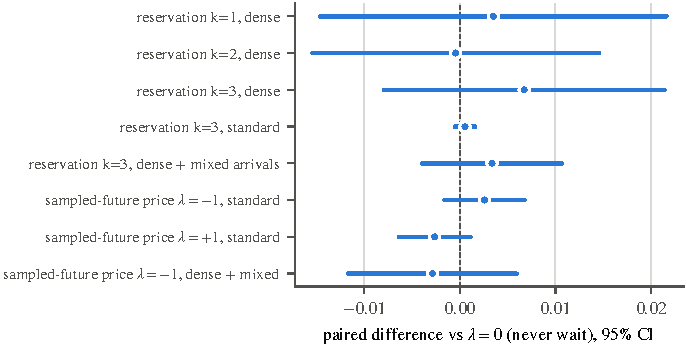
\includegraphics[width=0.72\linewidth]{figures/fig_q1.pdf}
\caption{Q1: waiting never helps. Paired differences of simple reservation and sampled-future prices against $\lambda=0$ (never wait), on standard worlds (seeds 201--230), dense stress worlds and an unseen arrival mixture (seeds 201--260).}
\label{fig:q1}
\end{figure}

\paragraph{Q1: Do sampled-future prices beat zero and simple reservation on unseen arrival mixtures and denser graphs?} \textbf{No} (Figure~\ref{fig:q1}).
\begin{itemize}
\item We built denser stress worlds (2--3 acceptable zones, ages $\pm12$, more multi-gender preferences), with about $3\times$ the introductions.
\item There, simple reservation ($k\in\{1,2,3\}$) and sampled-future prices are never distinguishable from $\lambda=0$. The same holds on an unseen arrival mixture (40\% on day 0, the rest over days 1--40).
\item The sign is instructive: keeping scarce members free ($\lambda<0$, our Round~1 intuition) beats prioritising them ($\lambda>0$), but neither beats acting now.
\item An introduction blocks people for only 8 days, and outcomes are driven more by individual tendencies than by pair fit, so a skipped pair is rarely recovered by a better one.
\end{itemize}

\paragraph{Q2: Does the policy generalise when conditions overlap or change, without recognising the scenario?} \textbf{Yes.} We built world variants by wrapping the generator and subclassing the simulator, without editing the kit. Against greedy (seeds 201--260), \full{} scores:
\begin{itemize}
\item $+0.0123$ \ci{+0.004}{+0.021} when conditions switch on day 30 to drift-style acceptance and delayed dates;
\item $+0.0079$ \ci{-0.002}{+0.018} with mixed arrivals;
\item $-0.0006$ with sparse and delayed conditions together, where there is nothing to choose between;
\item $+0.0065$ \ci{+0.002}{+0.011} overall.
\end{itemize}
We dropped Round~1's scenario classifier (the rules forbid family-specific logic); the online fit model provides continuous adaptation instead.

\paragraph{Q3a: Can complementary questions defeat an independent-item planner?} \textbf{Yes, in principle; ours avoids the trap.}
\begin{itemize}
\item In 90 initial pools we found 953 truly compatible pairs blocked by \emph{both} members' missing hard fields. Asking either member alone makes 0 of them feasible, so an independent-item planner values each half at exactly zero.
\item Such pairs are $22\%$ of all feasible pairs, and $43\%$ in cold start.
\item Our partner-count score treats unknown fields as possibly compatible, so both halves score positively. Every such pair had both members asked, and the median wait from co-presence to unlock fell from 6 to 4 days compared with list order.
\end{itemize}

\paragraph{Q3b: Do response penalties leave members waiting disproportionately?} \textbf{No.} The shipped person model down-weights observed non-responders. On seeds 341--380:
\begin{itemize}
\item served shares by true response-rate tercile (low, mid, high) are $33.7\%$, $34.3\%$ and $33.6\%$, against $33.5\%$, $34.2\%$ and $33.4\%$ for greedy;
\item members with over $50\%$ observed non-responses wait median/p90 $5/17$ days, against $6/20$ under greedy.
\end{itemize}
The penalty only breaks ties between equally large matchings: it reorders who goes first, but never removes anyone from the graph.

% ======================================================================
\section{Discussion: Round~1 hypotheses meet the evidence}\label{sec:discussion}

\begin{table}[t]
\centering\small
\caption{The Round~1 BRVM hypotheses, judged by Round~2 evidence.}
\label{tab:hyp}
\begin{tabularx}{\linewidth}{@{}lXX@{}}
\toprule
& Round~1 hypothesis & Round~2 verdict \\
\midrule
H1 & Global max-weight matching beats greedy ranking & \textbf{Only with soft-fit weights.} Unit weights $-0.005$; with quality weights, parity alone and essential inside the full policy \\
H2 & Reservation values (waiting) improve \msmi & \textbf{Rejected.} Never distinguishable from $\lambda=0$, even in dense worlds and unseen arrival mixtures (Q1) \\
H3 & Thompson sampling improves learning & \textbf{Not built, deliberately.} Each pair can be introduced once and nearly every feasible edge is used anyway, so exploration has little to change \\
H4 & Value-of-information questions beat random/none & \textbf{Supported in spirit.} Cheap proxies (likely-partner count; ask only when there are $\geq2$ options) are cost-efficient; no questions loses $71\%$ \\
H5 & Online updates and scenario adaptation help under change & \textbf{Supported without classification.} The online fit adapts in shifted worlds (+1.7\% skill), and the policy keeps its gain when conditions switch (Q2) \\
H6 & Correlated reciprocal acceptance improves ranking & \textbf{Not tested at policy level.} The shared shock is modelled exactly in our yardstick \\
H7 & A scarcity bonus raises coverage cheaply & \textbf{Rejected.} Slot prices change neither coverage ($0.325$ vs $0.324$) nor \msmi \\
\bottomrule
\end{tabularx}
\end{table}

Table~\ref{tab:hyp} grades our Round~1 proposal against the evidence.
\begin{itemize}
\item The parts that survived are the \emph{simple} parts of the proposal: reciprocal feasibility as a hard constraint, global matching, value-of-information-style questioning, and Bayesian shrinkage of person-level effects.
\item The parts that were cut (lookahead prices, exploration, scenario classification) all address headroom that the measurements show is not there.
\end{itemize}
The broader lesson for sequential reciprocal matching is that a validated, low-variance evaluator should come before any modelling ambition. Without it, every effect in this report would be invisible against noise roughly ten times larger.

% ======================================================================
\section{Limitations and broader impact}\label{sec:limits}

\begin{itemize}
\item \textbf{The worlds are synthetic.} Every finding (the low headroom, the value of goal and pace questions, the uselessness of waiting, the tie-breaking effect) is a claim about one published simulator with invented coefficients, not about people.
\item \textbf{The yardstick inherits the public simulator's structure.} Private worlds from a compatible engine may differ.
\item \textbf{The priors are hand-set.} The hand-set fit prior and the $+10$ arrival bonus are heuristics tuned on development seeds.
\item \textbf{The ranking is noisy.} At about $\pm0.04$ per team on 120 episodes, the realised-\msmi{} ranking cannot reliably separate competent policies whose expected scores differ by about $0.01$.
\item \textbf{Product use needs more.} Any authorised deployment would need real-time constraint checks, priors re-estimated and recalibrated on consented data, fairness review across protected groups, and a human in the loop.
\end{itemize}

\paragraph{Reproducibility and attribution.} The policy is deterministic and uses only the Python standard library; there are no trained assets and no external data. All commands, seeds and machine-readable results are in the repository. Claude Code (Anthropic) assisted with code, experiments and drafting under the team's direction; the team designed the approach, ran every evaluation and is responsible for all conclusions.

\begin{thebibliography}{9}\small
\bibitem{edmonds1965paths} J.~Edmonds. Paths, trees, and flowers. \emph{Canadian Journal of Mathematics}, 17:449--467, 1965.
\bibitem{hagberg2008networkx} A.~Hagberg, D.~Schult, and P.~Swart. Exploring network structure, dynamics, and function using NetworkX. In \emph{Proc.\ 7th Python in Science Conference (SciPy)}, 2008.
\bibitem{robbins1956empirical} H.~Robbins. An empirical Bayes approach to statistics. In \emph{Proc.\ Third Berkeley Symposium on Mathematical Statistics and Probability}, 1956.
\bibitem{gelman2013bayesian} A.~Gelman, J.~B.~Carlin, H.~S.~Stern, D.~B.~Dunson, A.~Vehtari, and D.~B.~Rubin. \emph{Bayesian Data Analysis}, 3rd ed. CRC Press, 2013.
\bibitem{vaswani2017attention} A.~Vaswani, N.~Shazeer, N.~Parmar, J.~Uszkoreit, L.~Jones, A.~N.~Gomez, {\L}.~Kaiser, and I.~Polosukhin. Attention is all you need. In \emph{Advances in Neural Information Processing Systems}, 2017. (Title homage only.)
\end{thebibliography}

\end{document}
